\chapter{睡眠和觉醒} \label{chap:chap44}

睡眠是一种非凡的状态。
它占据了我们生命的 1/3(平均寿命约为 25 年),但我们对大脑在日常活动中发生的事情知之甚少。
或许更令人惊讶的是,睡眠和做梦(睡眠中更值得注意的组成部分之一)的确切功能仍然未知。


尽管从\textit{柏拉图}和\textit{亚里士多德}到\textit{西格蒙德$\cdot$弗洛伊德},梦的心理内容一直是一个丰富的推测主题,但我们仍然不明白梦是否像\textit{弗洛伊德}假设的那样,具有深刻的个人意义,或者像\textit{弗朗西斯$\cdot$克里克}所说的那样,代表着大脑“扔掉垃圾”,即扔掉不值得保留的日常经历的点点滴滴。
睡眠的一个功能可能是允许突触重塑和巩固反映当天经历的记忆痕迹,但梦在这个过程中的作用仍然是一个激烈争论的话题。


在研究睡眠和觉醒时,研究人员通常使用\textit{多导睡眠图},它由三种生理指标组成:
通过\textit{脑电图}测量的大脑活动(图~\ref{fig:58_1})、通过\textit{眼电图}记录的眼球运动和肌肉、通过\textit{肌电图}测量的肌张力(图~\ref{fig:44_1}B)。
因为许多睡眠障碍患者在睡眠期间呼吸中断,所以在临床多导睡眠图中还测量呼吸。


\begin{figure}[htbp]
	\centering
	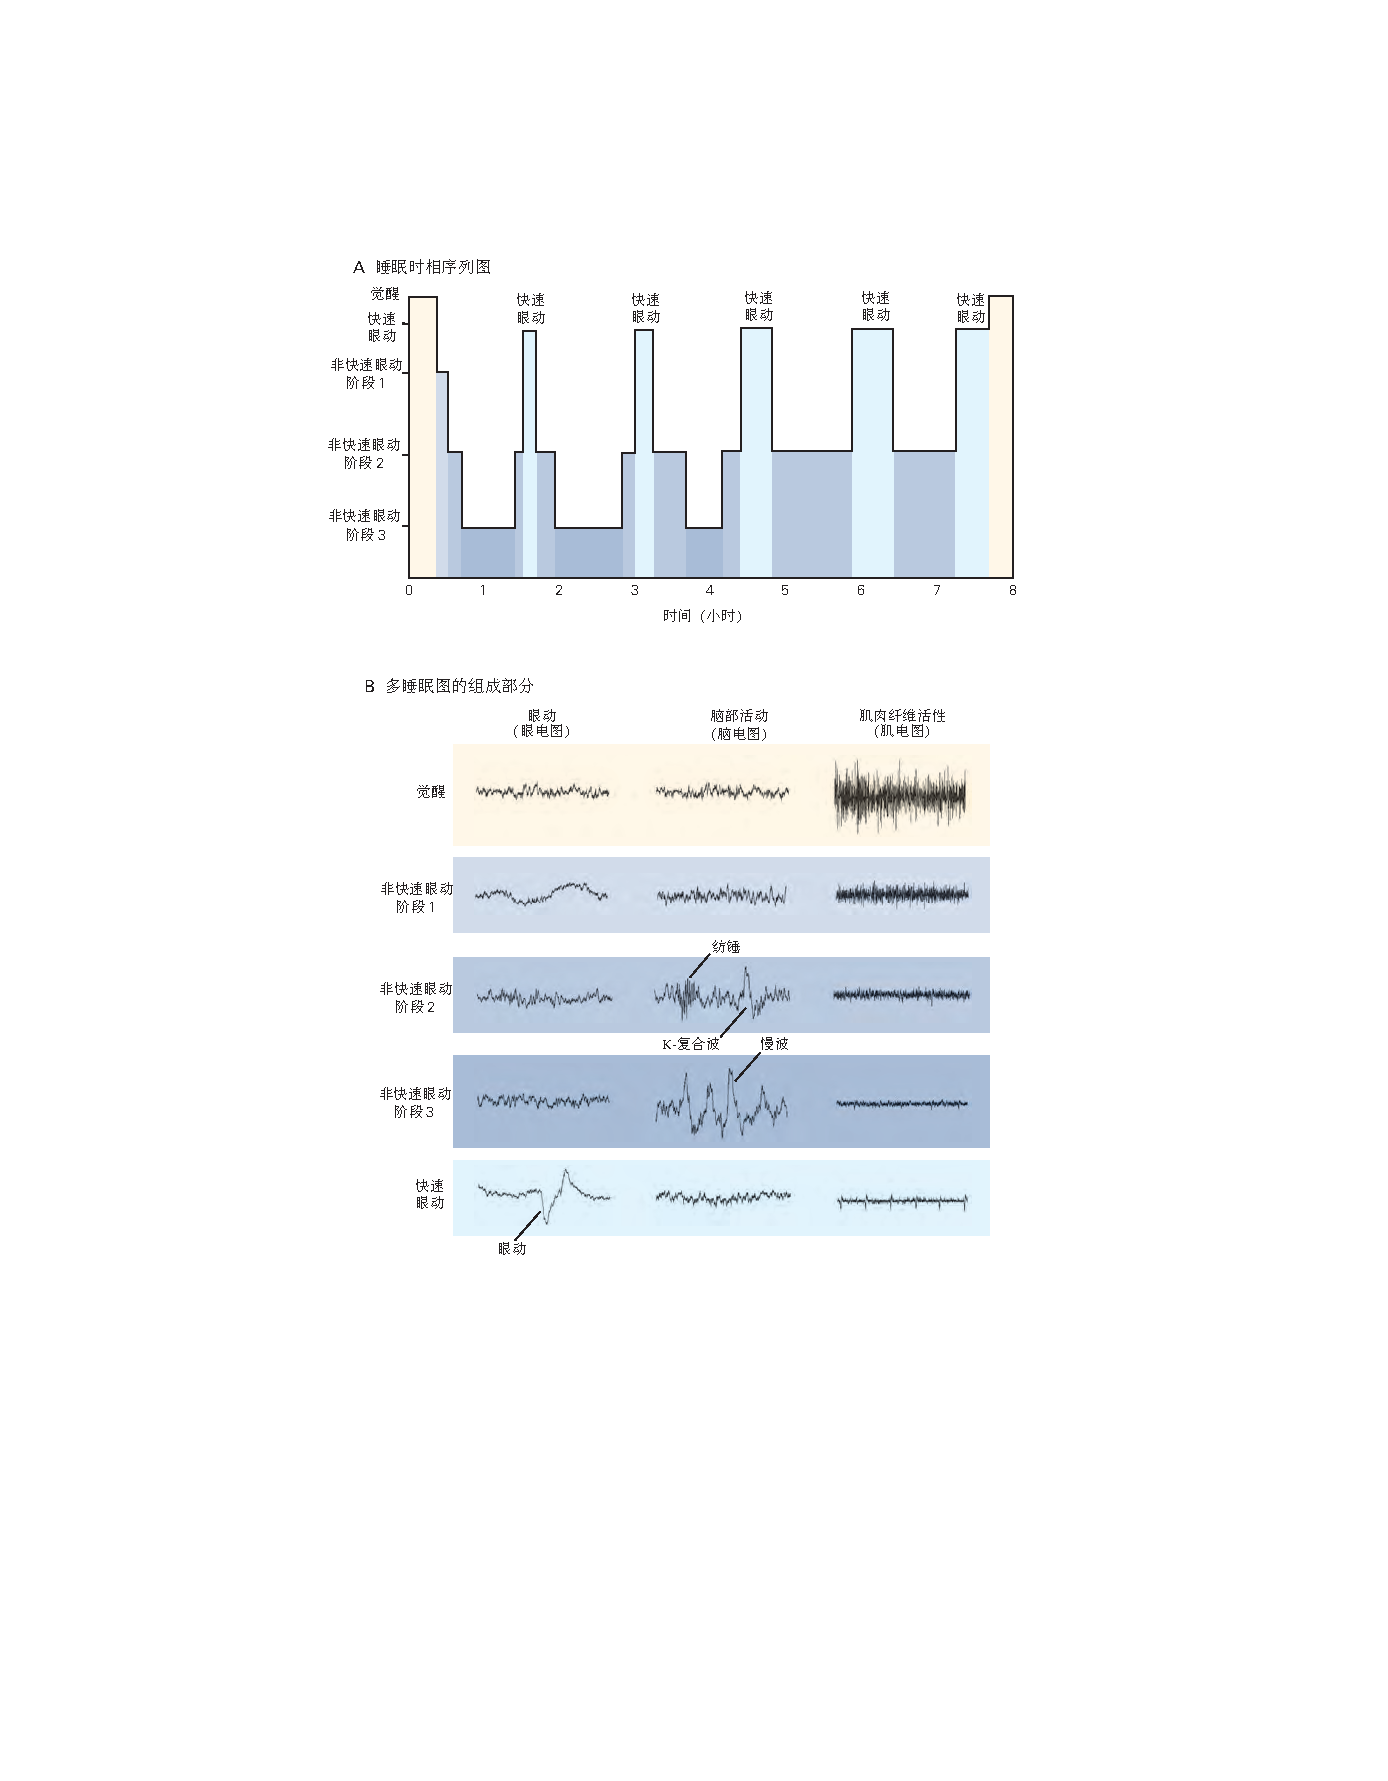
\includegraphics[width=0.75\linewidth]{chap44/fig_44_1}
	\caption{觉醒和睡眠的电生理模式。
		A. 一张睡眠时相序列图或图表,显示健康年轻人在典型夜晚的睡眠阶段进展。
		\textit{快速眼动}睡眠周期与\textit{非快速眼动}睡眠周期大约每 90 分钟交替一次。
		一个人通常会从觉醒状态进入浅度\textit{非快速眼动阶段 1}睡眠,然后逐渐进入更深的非快速眼动睡眠(\textit{非快速眼动阶段 2}、\textit{非快速眼动阶段 3}),然后在第一阶段快速眼动睡眠发生之前回到较浅的非快速眼动睡眠(浅蓝色条)。
		随着夜晚的推移,个体在非快速眼动睡眠的最深阶段花费的时间越来越少,而\textit{快速眼动}睡眠期的持续时间会增加。
		B. 记录显示用于区分睡眠阶段的多导睡眠图的组成部分。
		\textit{眼电图}通过眼睛两侧的电极记录眼球运动。
		\textit{脑电图}记录头皮的皮层场电位;\textit{肌电图}记录通过皮肤的肌肉纤维放电。
		在觉醒状态下,\textit{眼电图}显示自主眼球运动,\textit{脑电图}显示快速低振幅活动,\textit{肌电图}显示可变肌张力。
		\textit{非快速眼动阶段 1} 睡眠的特点是脑电图频率略有减慢,眼球运动缓慢,肌电图活动较少;
		\textit{非快速眼动阶段 2} 的特点是爆发 12 至 14 赫兹的活动,称为睡眠纺锤波和称为 K 复合波的高压慢波;
		\textit{非快速眼动阶段 3}以高压慢波为主。
		在快速眼动睡眠期间,脑电图与觉醒状态相似。
		在\textit{眼电图}上可以看到快速的眼球运动,但\textit{肌电图}非常安静,有时可以看到微小的心电图信号的污染(如图所示)。}
	\label{fig:44_1}
\end{figure}


在觉醒期间,脑电图以高频、低电压活动为主要特征,表明单个皮层神经元的独特活动;
\textit{眼电图}显示频繁的眼球运动;
肌电图显示中度和可变的肌张力。
在安静的觉醒状态下,闭眼时,$ \alpha $范围(8-13 赫兹)内的节律性脑电波很常见,尤其是在枕骨区域。
在睡眠的大部分时间里,脑电图显示出较慢的活动,但在夜间会周期性地转变为睡眠状态,脑电图速度更快、电压更低,肌张力下降,眼球快速运动称为\textit{快速眼动}睡眠。
如图~\ref{fig:44_1}~所示,从浅睡意到深度睡眠的整个缓慢脑电活动期称为非快速眼动睡眠,分为\textit{非快速眼动阶段 1}到\textit{非快速眼动阶段 3}三个阶段。



\section{睡眠包括交替的快速眼动睡眠和非快速眼动睡眠}

如图~\ref{fig:44_1}B~所示,当一个人变得昏昏欲睡并过渡到轻度非快速眼动睡眠(\textit{非快速眼动阶段 1})时,\textit{脑电图}变慢并显示出在 $ \theta $ 范围(4−7 赫兹)内的波。
意识在 \textit{非快速眼动阶段 1} 开始消退,但个体仍可能被最小的刺激唤醒。
\textit{非快速眼动阶段 2} 通常包含一些在 $ \theta $ 和 $ \delta $ 范围(0.5-4 赫兹)内的缓慢脑电图活动以及睡眠纺锤波,即持续 1 到 2 秒的 10 到 16 赫兹的渐强和渐弱脑电图振荡,通常逐渐开始和结束,因此脑电图波类似于两端逐渐变细的老式纺锤体。
如图~\ref{fig:44_1}B~所示,脑电图也可能显示大的单一慢波,称为 K-复合波。
在 \textit{非快速眼动阶段 3},脑电图显示出丰富的、非常缓慢的脑电$\delta$活动。
在 \textit{非快速眼动阶段 2} 和 \textit{非快速眼动阶段 3},由于缓慢的皮层活动扰乱了信息处理,人们通常对周围的世界没有意识。
在非快速眼动睡眠的所有阶段,眼球运动都消失了,肌肉张力低下,呼吸缓慢而规律,体温下降。


缓慢的\textit{脑电图}活动和睡眠纺锤波分别来自皮层-皮层和皮层-丘脑电生理相互作用。
在\textit{非快速眼动}睡眠期间,皮层锥体神经元的膜电位在向上状态(当它们去极化和放电时)和向下状态(当它们超极化和沉默时)之间波动。
膜电位的这些缓慢振荡甚至发生在孤立的皮层板中,与\textit{脑电图}中的慢波相关。
在 \textit{非快速眼动阶段 2} 睡眠,纺锤波由丘脑网状核神经元和丘脑皮层中继神经元相互作用产生。
丘脑皮层神经元在\textit{非快速眼动}睡眠期间通常超极化且不活跃,但网状丘脑神经元的抑制可导致低阈值 \ce{Ca^2+} 通道打开,从而驱动丘脑皮层神经元中的 \ce{Na+} 脉冲。
然后丘脑皮层神经元兴奋并募集更多的网状神经元,启动睡眠纺锤波的下一个周期。
如图~\ref{fig:44_2}~所示,这种抑制和兴奋模式大约每 100 毫秒重复一次,经过几个周期后,随着网状神经元的反应减弱,纺锤体活动减弱。


\begin{figure}[htbp]
	\centering
	\includegraphics[width=0.9\linewidth]{chap44/fig_44_2}
	\caption{睡眠期间脑电图节律的细胞机制。
		A. 在非快速眼动睡眠期间构成脑电图慢波基础的\textit{慢波振荡}是由大脑皮层内在的大量反复兴奋连接和抑制连接产生的。
		即使在孤立的皮层板中,慢波也会继续。
		当单个神经元超极化并且不放电时,来自此类神经元的细胞内记录在缓慢振荡期间显示有节奏的向下状态,当膜电位去极化更多并且神经元激发多个动作电位时与向上状态交替。
		这种同步放电会产生树突状电位波,在\textit{脑电图}中表现为慢波。
		B. 同样,在丘脑切片中,循环回路产生纺锤波。
		网状核神经元(灰色)中的脉冲使丘脑皮层中继神经元(红色)超极化,足以使低阈值(T 型)\ce{Ca^2+} 通道失活。
		随着超极化减弱,这些 \ce{Ca^2+} 通道打开,由此产生的 \ce{Ca^2+} 电流使中继神经元去极化,在 \ce{Ca^2+} 通道脉冲平台顶部产生短暂的 \ce{Na+} 通道脉冲。
		同时,随着中继细胞的持续爆发,其兴奋性输出在网状神经元中产生 T 型 \ce{Ca^2+} 通道脉冲,从而驱动另一次 \ce{Na+} 脉冲爆发。
		由此产生对中继细胞的反馈抑制启动了一个新的爆发周期。
		这种放电模式每秒重复 12 到 14 次,由此产生的到达皮层的丘脑皮层动作电位波在\textit{脑电图}中产生睡眠纺锤波。
		上部迹线显示了本地中继细胞群的动作电位。
		下部迹线显示抑制性突触后电位和来自单个中继细胞的脉冲;
		在这个缓慢的时间基础上,细胞内记录中的每个上行代表最多六个动作电位的爆发。
		正如轨迹所示,在纺锤波的每个周期中,单个中继神经元都不会达到脉冲阈值。
		因此,细胞外脉冲活动的幅度因周期而异,这取决于恰好激发哪些神经元以及它们与细胞外电极尖端的距离。
		然而,每次丘脑放电的爆发都会在皮层中产生一连串的兴奋性突触后电位,从而导致脑电图波与丘脑放电时间锁定\cite{bal1995synaptic}。}
	\label{fig:44_2}
\end{figure}


大约 90 分钟的睡眠后,人们通常会进入称为\textit{快速眼动}睡眠的阶段,在这个阶段,梦往往是生动的,有时是离奇的。
\textit{快速眼动}睡眠于 1953 年被发现,当时\textit{尤金$\cdot$阿瑟林斯基}和\textit{纳撒尼尔$\cdot$克莱特曼}观察到,在一个晚上的睡眠中,成年人会有几次不规则的\textit{双眼同向运动},当从这种状态中醒来时,大约 3/4 的受试者报告说梦中有视觉图像。


由于来自脑干的下行通路抑制了运动神经元,因此在快速眼动睡眠期间肌肉张力极低。
这种麻痹影响几乎所有运动神经元,除了那些支持呼吸、眼球运动和一些其他功能(如括约肌控制)的运动神经元。
正如本章后面所讨论的,这种对运动神经元的抑制是至关重要的,因为它阻止了梦境的实际实施。


在快速眼动睡眠期间,身体会经历许多额外的生理变化。
在非快速眼动睡眠期间,体温会下降,在快速眼动睡眠中,体温会进一步下降,因为热量的产生和维持是最小的。。
自动调节发生改变,心率和血压可能发生巨大变化。
此外,在快速眼动睡眠期间,男性会经历阴茎勃起,而女性会经历性唤起的生理迹象。


整个晚上,非快速眼动睡眠与快速眼动睡眠交替出现,每个睡眠周期大约需要 90 分钟。
如图~\ref{fig:44_1}A~所示,健康年轻人的睡眠通常始于快速进入 \textit{非快速眼动阶段 3}的\textit{非快速眼动}睡眠,接着是较浅的\textit{非快速眼动}睡眠,然后是一些\textit{快速眼动}睡眠,并且在每个周期中,非快速眼动睡眠变得\textit{更浅},快速眼动睡眠的\textit{周期变长}。
在睡眠期结束时,人们通常会从一段\textit{快速眼动}睡眠中自发醒来。



\section{上行的唤醒系统促进觉醒}

睡眠和觉醒神经基础的现代观点可以追溯到大约 100 年前由神经学家和神经病理学家\textit{康斯坦丁$\cdot$冯$\cdot$伊克诺莫}得出的概念。
第一次世界大战前后,他观察到一种不寻常的脑炎,被认为这是一种专门攻击睡眠-觉醒控制回路的脑部病毒感染。
在大多数情况下,患者患有“嗜睡性脑炎”,每天睡 20 小时或更长时间。
当他们醒来时,他们通常头脑清醒,但他们只会在吃饭时保持清醒,然后马上又睡着了。
这种强烈的困倦会持续好几个月才好转。
但在此期间死亡的患者中,\textit{冯$\cdot$伊克诺莫}在中脑和间脑的交界处发现了大脑的局灶性损伤,这使他假设上脑干和后下丘脑包含激活前脑的关键回路,产生正常的觉醒状态。


% Other patients afflicted in the same
受同一流行病影响的其他患者则面临完全相反的问题:持续的严重失眠。
他们会焦躁不安,尽管感到困倦,却无法入睡。
最终,他们每天只能睡几个小时,但醒来时并没有感到精神焕发。
在对这些患者进行尸检时,\textit{冯$\cdot$伊克诺莫}在下丘脑前部发现了病变。
他提出,该区域的神经元对于抑制脑干唤醒系统以允许睡眠很重要。
现代研究表明,大脑中的唤醒-睡眠回路系统非常接近\textit{冯$\cdot$伊克诺莫}的模型。



\subsection{脑干和下丘脑的上行觉醒系统支配前脑}

自\textit{冯$\cdot$伊克诺莫}时代以来,上行唤醒系统的组成一直存在争议。
在 20 世纪 40 年代末和 50 年代初,损伤研究证实,中脑上部网状结构的损伤可能导致昏迷,而对该区域的电刺激可能会唤醒动物。
\textit{觉醒促进神经元}的位置和性质是未知的。


在接下来的几十年里,很明显这些损伤损害了投射到前脑的上脑干神经元的轴突,包括蓝斑中的去甲肾上腺素能神经元、中缝背侧和中缝中的\textit{5-羟色氨}能神经元以及中脑多巴胺能神经元(第~\ref{chap:chap40}~章)。
如图~\ref{fig:44_3}~所示,下丘脑后部其他神经元的轴突,包括那些产生组胺和食欲素的神经元,也加入了这条通路,它分成两束,一些投射支配丘脑,另一些投射支配下丘脑、基底前脑和大脑皮层。


\begin{figure}[htbp]
	\centering
	\includegraphics[width=0.94\linewidth]{chap44/fig_44_3}
	\caption{上行唤醒系统。
		上行唤醒系统主要包括\textit{臂旁核}和被盖\textit{脑桥脚核}中的谷氨酸能神经元以及\textit{基底前脑}中的胆碱能神经元和\textit{$\gamma$-氨基丁酸能}(深灰色)神经元的轴突。
		\textit{臂旁核}和\textit{脑桥脚核}或\textit{基底前脑}的损伤会导致昏迷。
		不太重要的是\textit{腹侧被盖区}和\textit{中脑导水管周围灰质}中的多巴胺能神经元,以及\textit{乳头体上核}中的谷氨酸能和$\gamma$-氨基丁酸能神经元,这些部位的损伤可使睡眠增加约 20\%。
		此外,调节神经元群在受到刺激时可以强烈促进觉醒,但当受到损伤时,觉醒-睡眠量的变化很小。
		这些包括去甲肾上腺素能蓝斑中的单胺能神经元、5-羟色胺能背核和中缝核,以及组胺能结节乳头核;
		\textit{脑桥脚核}和外侧背侧被盖核中的胆碱能神经元;
		和\textit{外侧下丘脑}中的食欲素能神经元。
		所有这些神经元都将它们的轴突通过下丘脑和基底前脑直接送到大脑皮层,它们的净效应是增加皮层觉醒。
		许多调节通路也激活丘脑,使丘脑能够将感觉信息传递到大脑皮层。
		下丘脑外侧的\textit{$\gamma$-氨基丁酸能}神经元也通过抑制腹外侧视前区和丘脑网状核中的神经元来促进觉醒。}
	\label{fig:44_3}
\end{figure}


参与所有这些上行通路的神经元在觉醒状态下放电最快,但在睡眠期间要慢得多,这表明它们在促进觉醒。
然而,尽管许多单胺拮抗剂会引起嗜睡,并且单胺能细胞群的损伤会削弱在不利条件下保持觉醒的能力,但此类损伤对觉醒或睡眠数量或睡眠时间几乎没有持久影响。


% Lesions of the orexinergic neurons in the
外侧下丘脑食欲素能神经元的损伤会导致发作性睡病,这是一种睡眠-觉醒状态正常但不稳定的病症,如后文所述。
事实上,在被认为有助于觉醒的所有单胺能细胞群中,只有中缝背核附近的多巴胺能神经元的损伤会导致觉醒程度小而持久的减少,从而导致总睡眠时间增加约 20\%。
有趣的是,安非他明或莫达非尼等药物促进觉醒的能力似乎取决于它们阻断多巴胺再摄取的能力,因为多巴胺转运蛋白缺失的小鼠对这些药物没有反应。


% Because lesions of the ascending
由于上行单胺能和食欲素能通路的损伤对觉醒总时间几乎没有影响,最近的研究强调了谷氨酸能、胆碱能和\textit{$\gamma$-氨基丁酸能}神经元在维持觉醒中的作用。
背外嘴侧脑桥谷氨酸能神经元的损伤,包括\textit{臂旁核}和邻近的\textit{脚桥被盖核},导致动物无法从昏迷状态中醒来。
局限于丘脑的损伤会损害意识内容,但对觉醒-睡眠周期的影响相对较小。
另一方面,下丘脑后外侧的损伤会导致极度嗜睡,这不能用该区域食欲素能或组胺能神经元的损伤来解释。
乳头上区的谷氨酸能神经元激活皮层,下丘脑外侧的\textit{$\gamma$-氨基丁酸能}神经元抑制睡眠促进回路,可能是这种唤醒效应的原因。
最后,基底前脑的双侧大损伤也可造成昏迷,类似于背外侧脑桥的病变。
基底前脑中胆碱能、氨基丁酸能或谷氨酸能神经元的光遗传学或化学遗传学激活表明所有 3 种类型的神经元都可能产生觉醒。


因此,目前对上行唤醒系统的看法是:关键成分是背外侧脑桥、乳头上丘脑和基底前脑中的谷氨酸能神经元;
背外侧脑桥和基底前脑中的胆碱能神经元;
和下丘脑外侧和基底前脑中的\textit{$\gamma$-氨基丁酸能}神经元。
如图~\ref{fig:44_3}~所示,这些可能会被包含食欲素和单胺类的调节通路增强,需要允许完全和持续的觉醒,特别是在不利条件下。



\subsection{上行觉醒系统受损导致昏迷}

意识取决于觉醒状态下大脑半球的活动。
因此,当上行觉醒系统或双侧大脑半球受到损伤,或出现影响双侧觉醒系统的严重代谢紊乱(例如,低血糖、氧合不足、各种形式的药物中毒)影响觉醒系统及其皮层目标时,就会出现意识丧失。
患者即使受到强烈刺激也无法唤醒,称为昏迷。
那些可以被这种刺激部分唤醒的人被称为昏迷或迟钝。


对昏迷或反应迟钝患者的临床处理方法首先是确定上行觉醒系统是否有损伤。
由于唤醒通路与控制眼球运动和瞳孔反应以及呼吸和一些运动反应(第~\ref{chap:chap40}~章)的通路很接近,因此临床医生会仔细检查这些脑干功能。
如果这些功能完好无损,则问题很可能是由于代谢状况引起的,可以通过各种血液和脊髓液测试来评估。
此外,需要对大脑进行\textit{计算机断层扫描},以寻找影响两个大脑半球的病理(例如,大肿瘤或血块)。



\subsection{由相互抑制的神经元组成的回路控制从觉醒到睡眠和从\textit{非快速眼动}睡眠到\textit{快速眼动}睡眠的转变}

与昏迷相反,睡眠是一种暂时的、可逆的意识丧失,由抑制上行觉醒系统的特定大脑回路产生。
腹外侧视前核中的神经元含有抑制性神经递质\textit{$\gamma$-氨基丁酸}和甘丙肽,并广泛投射到上行觉醒系统的大部分。
这些视前神经元在觉醒时放电最慢,在动物入睡时放电增加,在睡眠剥夺一段时间后的深度睡眠期间放电最快。


同样,\textit{正中视前核}附近中的\textit{$\gamma$-氨基丁酸能}神经元也促进睡眠并投射到觉醒系统的某些组成部分。
这些视前神经元的损伤会导致睡眠碎片化,并导致动物失去多达一半的总睡眠。
与临床相关的是,老年人经常有睡眠碎片化,而那些睡眠碎片化程度最高的人在尸检中显示出促进睡眠的腹外侧视前甘丙肽神经元损失最大。
此外,面旁区(面神经附近的一个区域,因为它穿过脑干)中的大量\textit{$\gamma$-氨基丁酸能}神经元会抑制臂旁核。
面旁区的损伤也会导致多达一半的总睡眠时间损失。


有趣的是,\textit{腹外侧视前神经元}在整个唤醒系统中接收来自神经元的抑制性输入。
\textit{腹外侧视前神经元}和唤醒系统之间的相互抑制连接导致神经回路具有类似于电触发器开关的特性,其中回路的每一侧打开都会关闭另一侧。
这样的回路在两个状态之间产生快速和完全的转换。
虽然有时看起来入睡需要很长时间,但从觉醒到睡眠,或从睡眠到觉醒的实际转变,通常很快,只需要几秒钟到几分钟。
事实上,大多数动物几乎一整天都觉醒或睡着,很少有时间花在转换上。
这些快速转变在行为上具有适应性,因为动物在中间昏昏欲睡的状态下很脆弱。
如图~\ref{fig:44_4}~所示,神经触发器开关可防止这种情况发生,因为当开关的任一侧获得优于另一侧的优势时,回路会产生快速而完整的状态转换。


\begin{figure}[htbp]
	\centering
	\includegraphics[width=0.95\linewidth]{chap44/fig_44_4}
	\caption{促进睡眠的通路。
		A. 如图~\ref{fig:44_3}~所示,上行觉醒系统的组成部分从促进睡眠的神经元接收抑制性的、主要是\textit{$\gamma$-氨基丁酸能}的输入。
		\textit{腹外侧视前核}和\textit{视前正中核}中的神经元支配整个觉醒促进系统,而\textit{面神经旁核}中的神经元主要支配臂旁区域。
		许多\textit{腹外侧视前核}神经元还含有\textit{甘丙肽}(一种抑制肽)。
		如图~\ref{fig:44_5}~所示,\textit{外侧下丘脑}中释放\textit{黑色素浓缩素}的神经元可通过抑制附近的食欲能神经元以及导水管周围灰质中阻止\textit{快速眼动}睡眠的神经元来促进\textit{快速眼动}睡眠。
		B. \textit{腹外侧视前核}和\textit{正中视前核}与上行觉醒系统相互抑制成分的触发器开关关系。
		当被激活时,促进睡眠的神经元会抑制上行觉醒系统的组成部分。
		然而,促进睡眠的细胞群也受到觉醒系统的抑制。
		最终效果是个人大部分时间都处于完全觉醒或睡眠状态,同时最大限度地减少过渡状态的时间。}
	\label{fig:44_4}
\end{figure}


\begin{figure}[htbp]
	\centering
	\includegraphics[width=0.84\linewidth]{chap44/fig_44_5}
	\caption{\textit{快速眼动}睡眠开关。
		脑干神经元对于控制\textit{非快速眼动}和\textit{快速眼动}睡眠之间的转换至关重要。
		\textit{快速眼动}睡眠是由脑桥头端的一群神经元产生的,就在背侧被盖核和蓝斑的腹侧,在啮齿动物中称为亚侧背区,在人类中称为蓝斑下区。
		这些谷氨酸能神经元投射到脑干的其他部分,在那里它们启动\textit{快速眼动}睡眠的运动和自动表现,并投射到前脑,在那里它们调节\textit{快速眼动}睡眠的行为和脑电图成分。
		下行投射激活髓质和脊髓中的抑制性中间神经元,使运动神经元极化并阻止个体实现他梦中所想。
		如图~\ref{fig:44_4}B~所示,这些\textit{快速眼动开启}神经元被腹外侧导水管周围灰质和邻近的脑桥网状结构中的 \textit{$\gamma$-氨基丁酸能}神经元抑制,而后者本身被\textit{快速眼动开启}区域的神经元抑制,从而形成触发器开关。
		这些\textit{快速眼动关}神经元受前脑神经元控制,包括释放兴奋性食欲素神经肽的神经元、释放抑制性信号分子\textit{$\gamma$-氨基丁酸}和甘丙肽的\textit{腹外侧视前核}神经元,以及释放抑制性神经肽\textit{黑色素浓缩素} 的下丘脑神经元。
		此外,蓝斑和中缝背侧的调节神经元会抑制快速眼动生成器,而\textit{脑桥脚核}和背侧被盖核中的胆碱能神经元会促进快速眼动睡眠。
		该模型解释了许多临床观察结果,例如胆碱能激动剂药物促进快速眼动睡眠,而增加单胺水平的抗抑郁药等药物抑制快速眼动睡眠。
		食欲能神经元的缺失会导致快速眼动睡眠突然开始,而背侧下区域的快速眼动启动神经元缺失会消除快速眼动睡眠期间的张力缺失。
		因此,患有这种疾病的人会在梦中表演(\textit{快速眼动}睡眠行为障碍)。}
	\label{fig:44_5}
\end{figure}


\textit{快速眼动}睡眠是由以脑桥为中心的脑干神经元网络产生的。
\textit{快速眼动}睡眠的快速脑电图节律和梦境活动被认为是由蓝核下区域(脑桥蓝斑腹侧)的谷氨酸能神经元以及支配基底前脑和丘脑。
其他谷氨酸能\textit{蓝斑下核}神经元通过投射到腹内侧延髓和脊髓产生\textit{快速眼动}睡眠麻痹,在那里它们激活\textit{$\gamma$-氨基丁酸能}和甘氨酸能神经元,使运动神经元深度超极化。


% The subceruleus area in turn receives input from
蓝核下区域依次接收来自导水管周围灰质内和旁边的一群\textit{$\gamma$-氨基丁酸能}神经元的输入,脑导水管在此处通向第四脑室。
这些神经元在觉醒和非快速眼动睡眠期间最活跃,它们会抑制\textit{蓝斑下核},阻止进入快速眼动睡眠。
相反,蓝绿色下区域的\textit{$\gamma$-氨基丁酸能}神经元也投射回腹外侧导水管周围灰质。
两个神经元群之间的相互抑制可能会形成另一个触发开关,促进快速、完全地进入和退出\textit{快速眼动}睡眠。


有趣的是,去甲肾上腺素能的蓝斑和\textit{5-羟色氨}能的中缝背核支配并抑制蓝斑下区域。
因此,当人们服用会增加大脑\textit{5-羟色氨}或去甲肾上腺素水平的抗抑郁药时,\textit{快速眼动}睡眠通常会减少。
此外,如图~\ref{fig:44_5}~所示,由于这些单胺能神经元在觉醒期间很活跃,它们会阻止从觉醒直接过渡到\textit{快速眼动}睡眠。



\section{睡眠受稳态和昼夜节律驱动器调节}

睡眠的昼夜节律遵循 24 小时生物钟(稍后描述),而睡眠的稳态驱动力在觉醒状态下逐渐积累。
经过一段时间的睡眠剥夺后,大部分失去的睡眠会在接下来的几个晚上恢复,这在年轻人中可能涉及更深和更长的 \textit{非快速眼动阶段 3} 睡眠。


\textit{快速眼动}睡眠在\textit{快速眼动}剥夺后也会恢复;
反弹的\textit{快速眼动}睡眠可能包括特别强烈的梦、长时间的\textit{快速眼动}睡眠,以及偶尔从\textit{快速眼动}睡眠现象中突破到觉醒状态,例如入睡或醒来时出现类似梦境的幻觉或短暂的麻痹。
对于那些在工作日早早醒来并错过最后一部分睡眠(主要是\textit{快速眼动}睡眠)的人来说,周末的反弹睡眠通常会有丰富的\textit{快速眼动}睡眠。



\subsection{睡眠的稳态压力取决于体液因素}

大脑中循环的体液因子发出非快速眼动睡眠的稳态压力信号。
大脑在觉醒期间的新陈代谢非常活跃并使用\textit{三磷酸腺苷},但在持续觉醒的情况下,\textit{三磷酸腺苷}被去磷酸化为腺苷,腺苷在细胞外环境中充当局部神经调节剂。
腺苷 1 型受体是抑制性受体,在促进觉醒的神经元和大脑的许多其他部位表达,因此较高的腺苷水平可能会通过抑制这些神经元而产生困倦。
此外,腺苷可通过腺苷 2a 型受体兴奋神经元;
这些受体在伏隔核的外壳中很常见,并且可能通过投射到激活\textit{腹外侧视前神经元}的下丘脑来引起困倦。


睡眠压力可以通过一个人在舒适的环境中入睡所需的时间来衡量。
睡眠临床医生在多次睡眠潜伏期测试中使用了这种方法,其中从上午 9 点开始,每 2 小时给一个人 20 分钟的时间间隔,尝试在舒适、安静的床上入睡,共进行 5 次睡眠。
一个休息良好的人通常至少需要 15 到 20 分钟才能入睡,但一个非常困倦的人每次小睡只需几分钟即可轻松入睡。
另一个睡眠压力测试是心理运动警戒任务。
受试者被告知要注视一盏小灯,并在看到灯亮起后立即按下按钮。
然后,在 5 到 10 分钟的测试期间,灯会随机点亮;
昏昏欲睡的受试者注意力不集中,间歇性地对光刺激反应缓慢或完全没有反应。



\subsection{昼夜节律由视交叉上核的生物钟控制}

昼夜节律是大致 24 小时的生理节律,使动物的内部状态与外部日常环境同步,并预测每天发生的各种生理需求。
在人类中,白天的昼夜节律唤醒信号抵消了不断上升的稳态睡眠压力。
昼夜节律唤醒信号在午后略有下降,此时许多人正在小睡或午睡。
在习惯性的就寝时间前后,这种昼夜节律的觉醒影响迅速瓦解,睡眠的稳态驱动力不受阻碍,睡眠随之而来。
如图~\ref{fig:44_6}A~所示,在习惯醒来时间之前的一两个小时内,昼夜节律会促进睡眠以确保充足的睡眠,因为睡眠后期的稳态睡眠压力较低。


\begin{figure}[htbp]
	\centering
	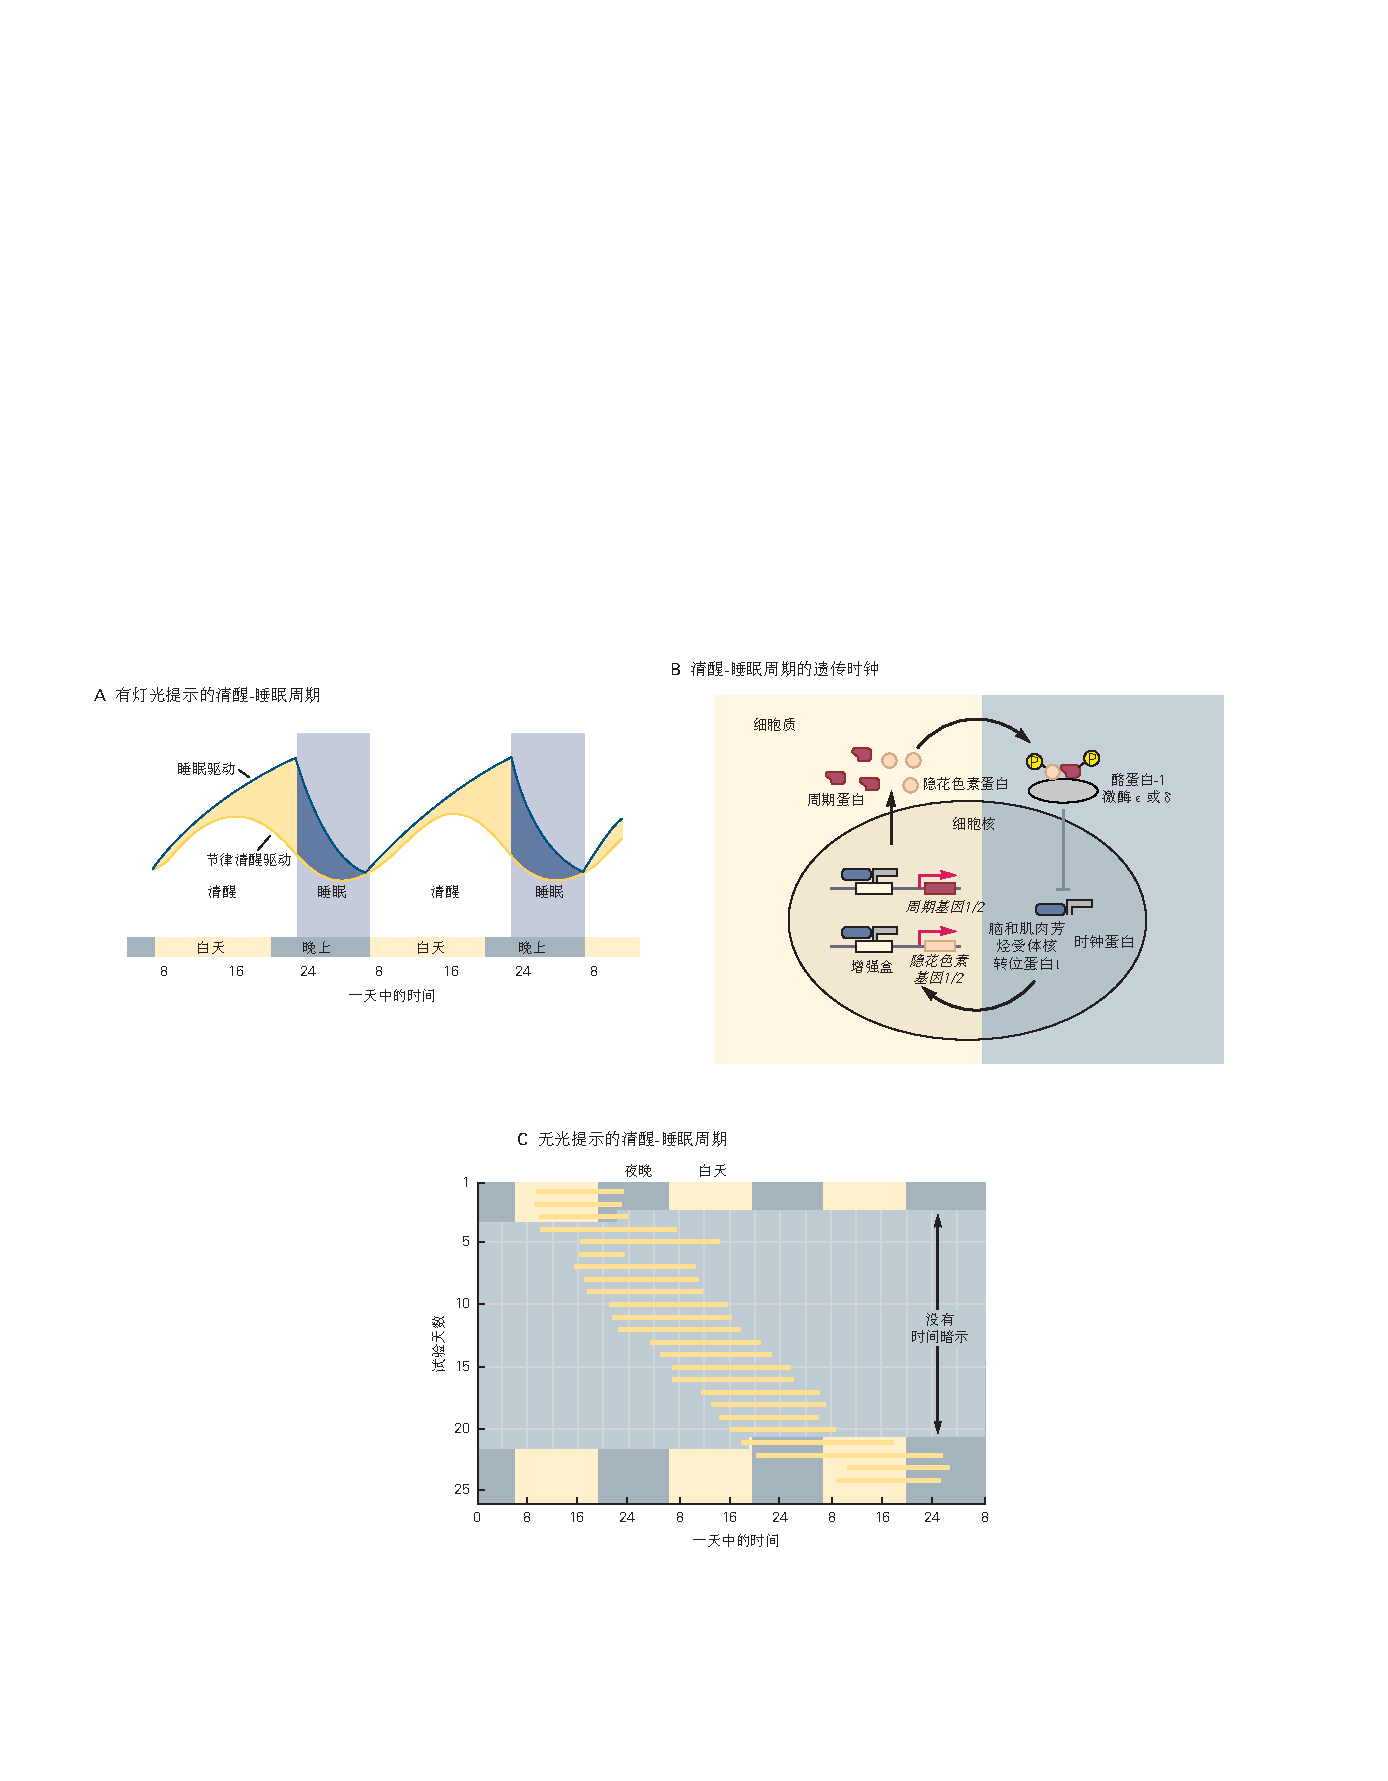
\includegraphics[width=1.0\linewidth]{chap44/fig_44_6}
	\caption{觉醒的昼夜节律驱动力与睡眠的稳态驱动力相互作用,形成觉醒-睡眠周期。
		A. 睡眠内驱力在长时间觉醒的过程中逐渐增强,而昼夜节律内驱力以 24 小时为周期变化,与之前的睡眠无关。
		这种昼夜节律觉醒周期的高峰出现在睡前几个小时,因为稳态睡眠驱动正在上升,而低点出现在习惯性觉醒时间之前的几个小时,此时睡眠的稳态驱动正在减弱。
		B. 哺乳动物细胞的 24 小时节律由一组形成转录-翻译环的蛋白质调节。
		\textit{脑和肌肉芳烃受体核转位蛋白1}和\textit{时钟蛋白}形成一个二聚体,与许多具有昼夜节律转录的基因上发现的\textit{增强盒}基序结合。
		其中包括\textit{周期基因 1} 和\textit{周期基因 2}和\textit{隐花色素基因 1} 和\textit{隐花色素基因 2}。
		他们的产物二聚化并与\textit{酪蛋白-1激酶$\epsilon$或$\delta$}形成复合物。
		该复合物易位至细胞核,在那里它抑制\textit{脑和肌肉芳烃受体核转位蛋白1}和\textit{时钟蛋白}的二聚化,导致它从\textit{增强盒}脱落。
		这减少了\textit{周期基因}和\textit{隐花色素基因}的转录;
		随着\textit{周期蛋白}和\textit{隐花色素蛋白}的降解,\textit{脑和肌肉芳烃受体核转位蛋白1}和\textit{时钟蛋白}再次二聚化,然后循环重复。
		C. 昼夜节律调节睡眠和觉醒的时间。
		该图显示了一个人的觉醒周期(黄色条),他最初在正常照明条件下生活了 3 天,然后在没有时间线索的昏暗环境中生活了 18 天。
		个体每天维持约 25.2 小时的周期,在此期间漂移一整天。
		如图~\ref{fig:44_7}~所示,无法将光信号传递到视交叉上核的盲人经常像这样连续生活,这种情况称为非 24 小时觉醒睡眠障碍。}
	\label{fig:44_6}
\end{figure}


\begin{figure}[htbp]
	\centering
	\includegraphics[width=0.7\linewidth]{chap44/fig_44_7}
	\caption{视交叉上核中的神经元为觉醒-睡眠提供了一个主时钟。
		视网膜输入光信号激活视交叉上核(上图),然后通过下丘脑中的一系列转发器驱动唤醒-睡眠周期(下图)。
		通过下丘脑的矢状切面显示视交叉上核投射到\textit{腹侧脑室下区}中的神经元,后者又投射到\textit{下丘脑背内侧核}。
		\textit{下丘脑背内侧核}含有谷氨酸能神经元,可刺激\textit{下丘脑外侧区}中的食欲能神经元和谷氨酸能神经元,从而引起觉醒。
		\textit{下丘脑背内侧核}中的\textit{$\gamma$-氨基丁酸能}神经元会抑制\textit{腹外侧视前核},从而关闭促进睡眠的系统。
		患有\textit{下丘脑背内侧核}病变的动物无法表现出昼夜节律,每天多睡一个小时左右。}
	\label{fig:44_7}
\end{figure}


% Circadian rhythms are driven by a small group
昼夜节律由位于视交叉正上方的下丘脑视交叉上核中的一小群\textit{$\gamma$-氨基丁酸能}神经元驱动。
这个生物钟的 24 小时活动节律由一组“时钟基因”驱动,这些基因经历一个大约 24 小时的转录-翻译周期。
该环的正肢由两种蛋白质组成,\textit{脑和肌肉芳烃受体核转位蛋白1}和\textit{时钟蛋白},它们二聚化并形成一个转录因子,与\textit{增强盒}基序结合,\textit{增强盒}基序存在于数百个基因的启动子区域,这些基因每天都在表达。
在\textit{脑和肌肉芳烃受体核转位蛋白1}和\textit{时钟蛋白}增加表达的那些基因中,有\textit{周期基因}和\textit{隐花色素基因}。
它们的蛋白质产物也二聚化,与\textit{酪蛋白-1激酶$\epsilon$或$\delta$}形成复合物,并转移到细胞核,在那里它们导致\textit{脑和肌肉芳烃受体核转位蛋白1}和\textit{时钟蛋白}从\textit{增强盒}解离,减少许多基因的转录,包括它们自身。
这导致\textit{周期蛋白}和\textit{隐花色素蛋白}下降,直到\textit{脑和肌肉芳烃受体核转位蛋白1}和\textit{时钟蛋白}可以再次二聚化,重新开始循环。
如图~\ref{fig:44_6}B~所示,除了这个核心循环之外,额外的遗传侧循环调节生物钟的周期。


% This daily gene cycle functions in almost
这种日常基因循环在身体的几乎所有细胞中发挥作用,包括大脑中的细胞,它对于驱动广泛的昼夜节律至关重要,从激素和消化酶的分泌到为肝脏做好食物代谢处理的准备,以及为一天的活跃时期做好心血管系统的准备。
当从身体中取出并放入培养皿中时,身体中的大多数细胞会迅速失去同步,因为细胞之间的个体细胞时钟周期与 24 小时平均值相差多达一两个小时。
然而,当培养视交叉上核的神经元时,它们会继续相互交流,从而同步它们的细胞节律。
视交叉上神经元的这种协调活动导致接近 24 小时的节律;
如图~\ref{fig:44_6}C~所示,处于连续昏暗光线环境中的人类的平均周期为 24.1 小时,导致昼夜节律缓慢漂移。


% The suprachiasmatic nucleus exerts
视交叉上核通过调节体温以及自主神经、内分泌和行为功能来控制所有其他生物钟。
有趣的是,虽然体温的每日节律可以调整许多器官节律的时间,但视交叉上核本身的节律对温度变化具有很强的抵抗力,因此其基本起搏没有改变。
最后,大脑和身体的昼夜节律时间取决于视交叉上时间。


尽管如此,视交叉上时钟必须被带到外部世界。
否则,每个 24.1 小时周期的人每天都会比前一天晚起 6 分钟,并且无法适应日出和日落的季节性变化。
为了避免这种情况,视交叉上核接收来自一类特殊的视网膜神经节细胞的直接输入,这些神经节细胞发出光水平信号,而不是参与图像形成。
像所有的视网膜神经节细胞一样,这些神经元接收来自视杆细胞和视锥细胞的输入,但它们也含有黑视蛋白,一种使它们本质上感光的感光色素,因此它们起到亮度检测器的作用。
除了在环境光周期中引入内部昼夜节律外,这些细胞还调节其他非图像形成视觉功能,例如瞳孔光反射和当人看亮光时可能出现的疼痛感。


由于时钟基因或其调节元件的突变,一些人的昼夜节律周期异常短。
例如,患有\textit{家族性睡眠时相提前综合症}的人喜欢在晚上早点睡觉,并且不能睡到凌晨 3 点或 4 点以后。
在患有这种疾病的家族中,编码\textit{周期基因}或\textit{酪蛋白-1激酶$\delta$基因}突变会导致时钟的更快速循环。


含有黑视蛋白的神经元受损的盲人缺乏对其视交叉上核的视觉输入,通常会导致非 24 小时睡眠-觉醒节律紊乱。
因为大多数人的内在周期都超过 24 小时,所以这些人的昼夜节律会漂移,每天晚几分钟,因此大部分时间他们与世界其他地方不同步。
由于视交叉上核缺乏来自视网膜的关键重置信号,它们缺乏适应外部明暗条件的能力。
这种问题在失去眼睛的人群中最为常见(例如由于创伤或感染),但在黑视蛋白神经元完整的盲人(例如由于视杆细胞和视锥细胞退化或角膜或晶状体问题而失明)且保留了\textit{瞳孔光反射}的盲人中并不常见。


% In contrast to light, which is
与黑视蛋白神经元发出的光信号相反,褪黑激素发出的是黑暗信号。
褪黑激素由松果体产生,视交叉上神经元通过与激活松果体交感神经支配的下丘脑室旁核中的神经元通讯来计时释放。
视交叉上核中的神经元含有褪黑激素受体,可增强昼夜节律。
同样,外源性褪黑激素或褪黑激素激动剂可以调节昼夜节律,通过调节入睡时间促进睡眠。
这种治疗方法对于在患有非 24 小时睡眠-觉醒节律障碍的个体中引入昼夜节律特别有用。



\subsection{睡眠的昼夜节律控制取决于下丘脑中继}

在所有哺乳动物物种中,视交叉上核在每天光照期间最为活跃。
人类是昼夜活动的(白天醒着,晚上睡着),而夜间活动的哺乳动物则具有相反的活动周期。
如果视交叉上核在光照期间最活跃,它如何设置这种相反的行为模式?


答案似乎在于在视交叉上核和唤醒-睡眠控制回路之间插入的一系列转发器,这使昼夜节律计时系统可以灵活地满足个人的需求。
视交叉上神经元是\textit{$\gamma$-氨基丁酸能}神经元,它们将大部分输出发送到称为室旁区的相邻区域。
下丘脑前部的这个区域主要包含与视交叉上核反相发射的\textit{$\gamma$-氨基丁酸能}神经元,即在夜间最活跃。
室旁区的目标在很大程度上与视交叉上核的目标重叠,包括调节各种生理和行为系统的脑室旁、背内侧、腹内侧和外侧下丘脑的部分。
那么,据推测,特定生理或行为功能的时间将取决于这两个反相昼夜节律输入与其目标神经元的关系。


室旁区的一个重要目标是下丘脑的背内侧核,它调节许多昼夜节律行为,包括觉醒-睡眠周期。
背内侧核的损伤会严重扰乱睡眠、进食、运动活动和皮层类固醇分泌的昼夜节律。
如图~\ref{fig:44_7}~所示,背内侧核被认为通过\textit{$\gamma$-氨基丁酸能}投射到腹外侧视前核和谷氨酸能投射到外侧下丘脑来促进觉醒。



\subsection{睡眠不足会损害认知和记忆}

当人们困倦时,他们的警觉性、工作记忆、判断力和洞察力往往会受损。
一些注意力问题可能是由\textit{微睡眠}引起的,\textit{微睡眠}是皮层活动短暂较慢的时期。
例如,受试者在充分休息时很少会错过心理运动警觉任务中的刺激,但在困倦时可能会错过超过 20\% 的视觉刺激。
除了皮层功能的这些整体失误之外,嗜睡还可以在局灶性皮层区域产生具有慢脑电波的局部睡眠。
执行功能通常是第一个因困倦而失败的事情,睡眠不足的人在脑电图中显示出新陈代谢减少和额叶皮层的局灶性减慢。


虽然困倦会损害认知,但睡眠本身有助于巩固记忆。
当受试者被教导一项简单的运动任务时,例如按预定顺序按下按钮,他们在练习中会变得更有效率。
\textit{罗伯特$\cdot$史蒂克戈德}及其同事发现,如果在早上进行训练,并且在晚上 12 小时后对受试者进行测试(没有干预睡眠),他们的表现与停止训练时的水平大致相同。
然而,如果他们在睡了一夜后第二天早上接受测试,他们的表现通常会比训练当天更好。
在晚上接受训练的受试者在 12 小时后仍然表现更好,如果他们有机会睡一夜,但如果他们保持觉醒则不会。
某些类型的记忆巩固(例如,视觉感知任务的记忆)的改善与\textit{快速眼动}睡眠的量相关,而其他类型(例如,手指敲击序列任务的记忆)与\textit{非快速眼动阶段 2} 睡眠相关。


这些研究表明,在睡眠的每个阶段,大脑皮层都会进行突触重组,以巩固对特定类型显著信息的记忆。
相反,当受试者睡眠不足或睡眠碎片化时,这种记忆巩固就会消失。
\textit{朱利奥$\cdot$托诺尼}和\textit{基娅拉$\cdot$奇雷利}提出的一个相关理论是:基于最近经验(突触稳态)的突触强度重新平衡发生在睡眠期间。
许多兴奋性突触的大小在学习过程中增加,需要减少一些兴奋性输入以避免过度兴奋目标神经元。
\textit{托诺尼}和\textit{奇雷利}发现,在睡眠期间,运动皮层和感觉皮层中较小的突触尺寸会减少,导致强输入得到加强,而竞争性较弱的输入被消除。


% Diseases that cause sleep loss or
导致失眠或使人从睡眠中醒来的疾病会损害认知能力。
例如,阻塞性睡眠呼吸暂停会严重破坏睡眠,导致白天嗜睡、注意力不集中和其他认知障碍。
睡眠碎片化在阿尔茨海默病中也很常见。
阿尔茨海默病患者的腹外侧视前核神经元往往较少,神经元丢失的程度与其睡眠碎片化程度相关。
治疗睡眠碎片化是否可以改善阿尔茨海默病患者的认知能力仍有待确定。



\section{睡眠随年龄变化}

睡眠会随着年龄的增长而发生显著和独特的变化。
每位新父母很快就会了解到,新生儿漫长的睡眠时间在一天中几乎是随机分布的。
尽管新生儿的脑电图节律不如大一点的儿童或成人形成得好,但超过 50\%(每天 8-9 小时)的睡眠是在与快速眼动睡眠很相似的状态下度过的。


% Sleep recordings from a premature infant
早产儿的睡眠记录显示出更高比例的类\textit{快速眼动}睡眠,这表明胎儿在子宫内一天中的大部分时间都处于大脑激活但运动受抑制的状态。
由于神经元活动会影响大脑功能回路的发育(第~\ref{chap:chap48}~和~\ref{chap:chap49}~章),因此有理由认为未成熟大脑在睡眠期间的自发活动促进了神经回路的发育。


到大约 4 个月大时,普通婴儿开始表现出与白天和黑夜同步的昼夜节律,这大大减轻了疲惫的父母。
总睡眠时间逐渐减少,到 5 岁时,孩子每晚可能要睡 11 个小时加上打盹,10 岁左右通常睡 10 个小时。
在这些早期阶段,睡眠很深;
\textit{非快速眼动阶段 3} 是突出的,脑电图中有大量的$ \delta $波。
因此,儿童不容易被环境刺激惊醒。


% With age, sleep becomes lighter
随着年龄的增长,睡眠变得更轻、更零散。
进入 \textit{非快速眼动阶段 3} 睡眠的时间百分比在整个成年期下降,到 50 到 60 岁时,\textit{非快速眼动阶段 3}完全消失并不罕见,尤其是男性。
这种向非快速眼动睡眠较轻阶段的转变导致自发觉醒次数增加 2 到 3 倍,并且更容易打乱睡眠。
包括失眠和睡眠呼吸暂停的许多睡眠障碍,随着年龄的增长而变得更加普遍,并且失眠很常见,通常是由于响应排空膀胱的神经信号而醒来,或者由于更年期症状或关节炎和其他疾病引起的不适。
为什么这种变化会随着年龄的增长而发生尚不清楚。
稳态睡眠压力看似正常,但产生深度非快速眼动睡眠的神经机制可能不太有效。


\section{睡眠回路的中断导致许多睡眠障碍}

\subsection{失眠可能是由唤醒系统抑制不完全引起的}


失眠是所有医学中最常见的问题之一,但潜在的神经生物学仍然是个谜。
失眠是指入睡困难或难以维持睡眠,从而影响第二天的生活功能。
慢性失眠患者的正电子发射断层扫描研究表明,睡眠期间大脑唤醒系统异常激活,脑电图通常显示持续的高频活动(15-30 赫兹),这通常仅在觉醒时可见。


此外,暴露于急性应激的大鼠在睡眠期间表现出高频脑电图活动,以及腹外侧视前核神经元和唤醒系统组件(如蓝斑和组胺神经元)的同步活动。
这种同时激活可以产生一种独特的状态,在这种状态下,脑电图显示与睡眠一致的慢波以及与觉醒状态一致的高频活动;
这或许可以解释为什么有些患者在多导睡眠图记录上看起来睡着了,但他们可能会感到觉醒。


临床上,失眠通常通过认知行为疗法来治疗,旨在减少过度觉醒和改善睡眠习惯。
一些患者可能会接受\textit{苯二氮卓类}药物和相关药物的治疗,这些药物会增强\textit{$\gamma$-氨基丁酸}的传输,因此可能有助于减少促进觉醒的大脑区域的活动。
其他患者受益于更直接地阻断唤醒系统的药物,例如抗组胺药。


\subsection{睡眠呼吸暂停碎片睡眠和损害认知}

睡眠呼吸暂停是最常见的睡眠障碍之一,影响了大约 5\% 的成人和儿童。
患有阻塞性睡眠呼吸暂停的患者会反复发作气道阻塞,迫使患者从睡眠中短暂醒来以恢复呼吸。
在睡眠期间,肌张力下降,对于气道狭窄的人,气道扩张肌如\textit{颏舌肌}(通常用于向前拉动舌头)松弛会导致气道塌陷。
这会导致短时间内没有空气流动,因此,血液中的二氧化碳水平会升高,而氧气水平会下降,从而激活髓质中的化学感应系统,从而增加呼吸努力。


这些化学感觉系统还会激活臂旁核中的神经元,从而促进觉醒,从而进一步增加肌肉张力,从而重新打开气道。
这些气道阻塞每晚可能发生数百次,但觉醒通常非常短暂,以致于患者在早上可能不记得它们。
许多患有阻塞性睡眠呼吸暂停症的人早上感觉不到休息;
他们整天都感到困倦,并且难以完成各种各样的认知任务,尤其是那些需要保持警惕或学习的任务。


临床医生经常使用\textit{持续气道正压}设备治疗睡眠呼吸暂停,该设备通过鼻子输送适度加压的空气,在睡眠期间充气并打开气道。
睡眠呼吸暂停也可以通过上呼吸道手术来治疗,以去除大扁桃体等阻塞物,使用牙科设备来向前移动舌头,或者减轻体重以减少颈部的脂肪组织。
如图~\ref{fig:44_8}~所示,接受治疗的患者通常会感觉更加警觉并且具有更好的认知功能,尽管可能存在一些残余的认知障碍,这可能是由于反复发作的低氧饱和度或缺氧引起的神经元损伤。


\begin{figure}[htbp]
	\centering
	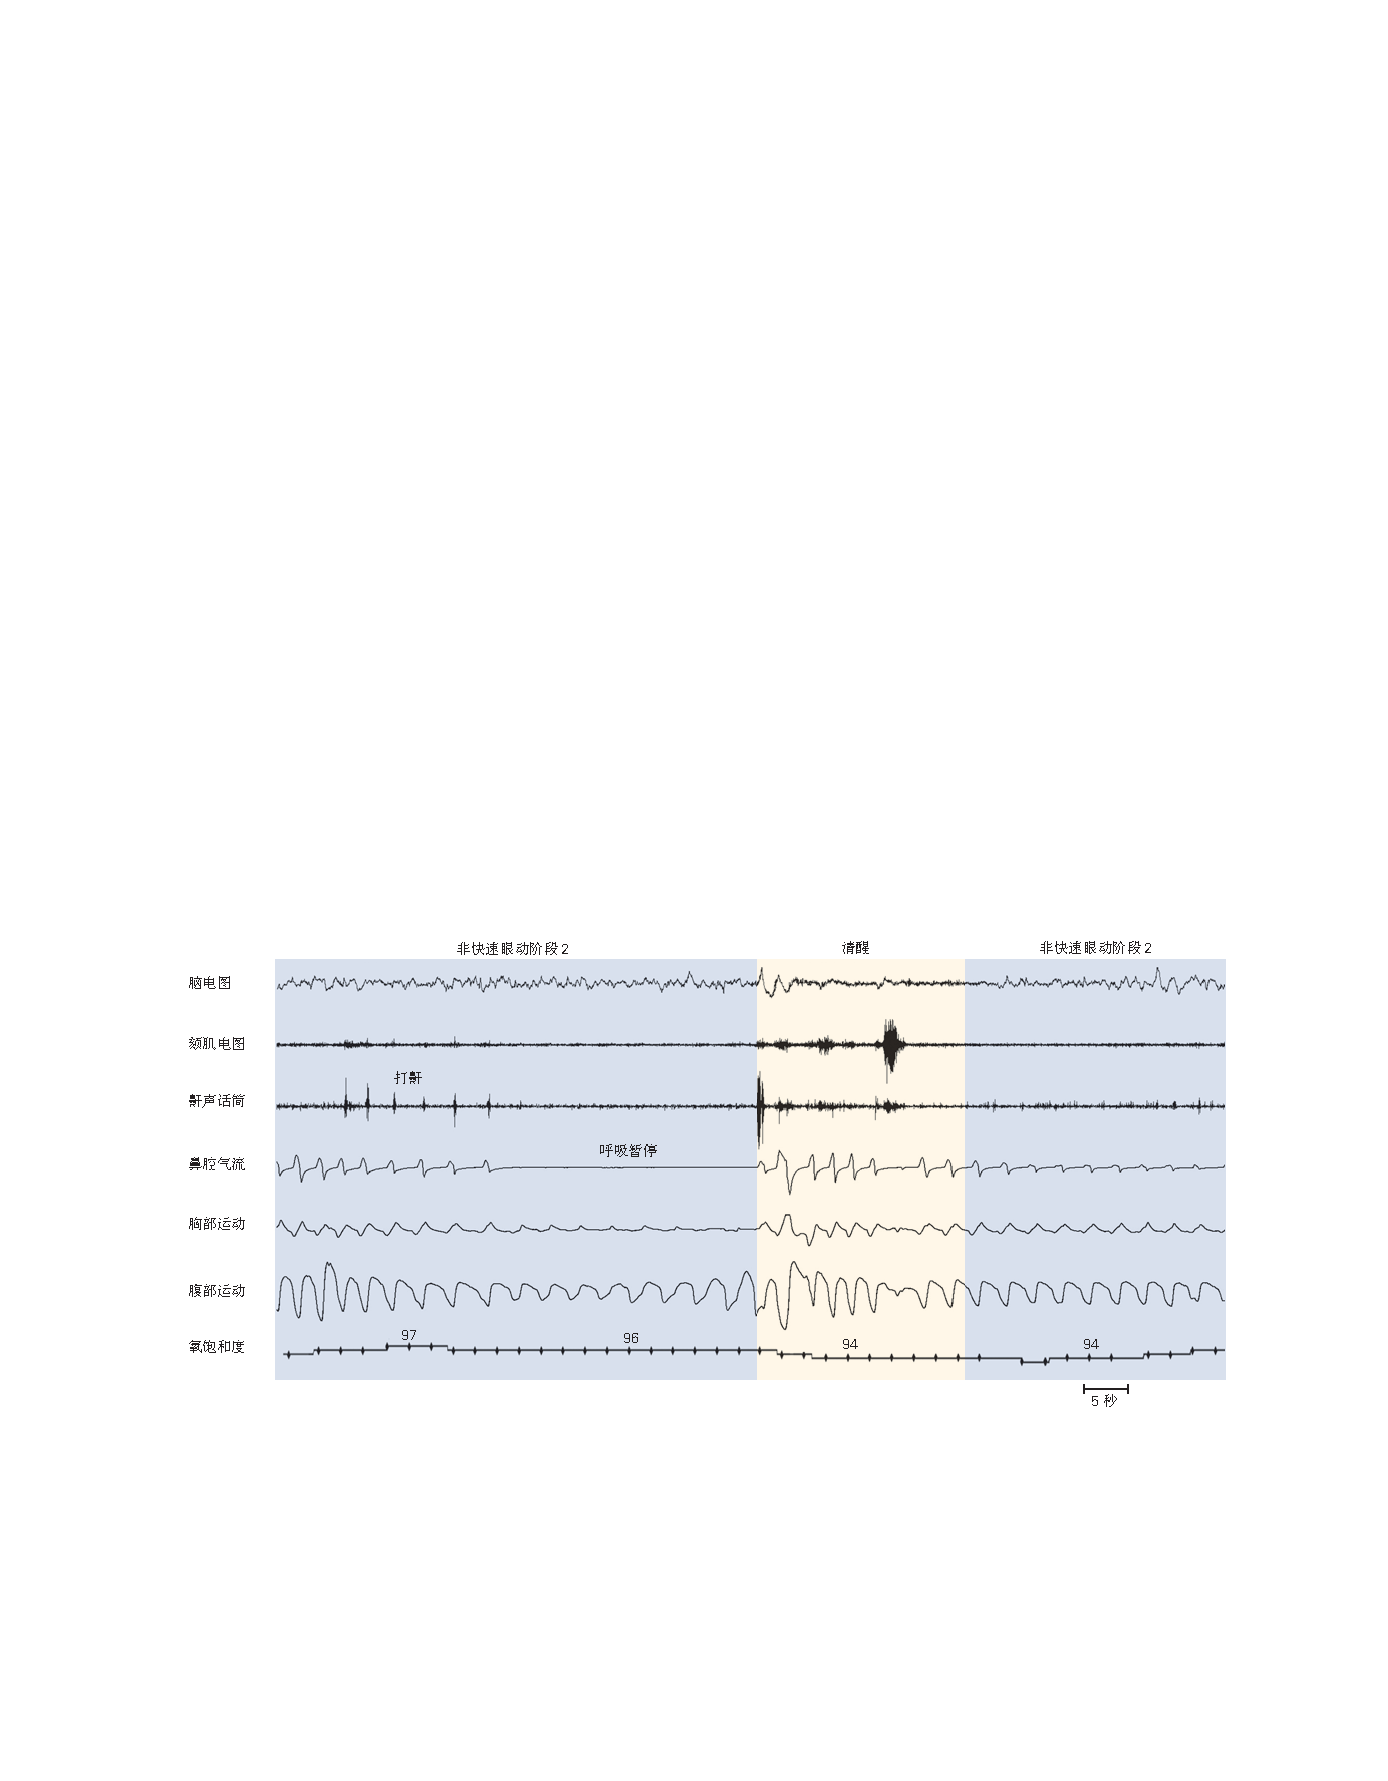
\includegraphics[width=1.0\linewidth]{chap44/fig_44_8}
	\caption{睡眠呼吸暂停发作。
		在这个多导睡眠图的开始,一个人处于 \textit{非快速眼动阶段 2} 睡眠。
		检测到一些打鼾,但鼻腔气流良好且氧饱和度正常。
		然后,个体会出现阻塞性呼吸暂停,没有鼻腔气流;
		然而,呼吸努力仍然存在(由腹部运动显示)。
		呼吸暂停由短暂的觉醒(低电压快速脑电图)终止,伴随着响亮的鼾声、肌电图活动增加、呼吸努力增强和气道开放。
		氧饱和度下降约 3\%,在呼吸暂停结束约 15 秒后达到最低点,因为血液从肺部流到测量氧饱和度的指尖需要时间。}
	\label{fig:44_8}
\end{figure}


\subsection{发作性睡病是由食欲神经元的缺失引起的}

发作性睡病最早是在 1800 年代末被描述的,但其根本原因(单一神经递质的缺乏),直到最近 20 年才变得清晰。
发作性睡病通常始于青少年时期,表现为每天中度至重度嗜睡,即使晚上睡眠充足。
发作性睡病患者很容易在课堂上、开车时或在其他睡眠可能令人尴尬或危险的活动中睡着。
与睡眠呼吸暂停不同,他们的睡眠是恢复性的,在小睡 15 到 20 分钟后,他们通常会感觉更加觉醒。


此外,在发作性睡病患者中,\textit{快速眼动}睡眠的要素通常发生在觉醒期间。
例如,在夜间入睡或醒来时,发作性睡病患者可能会发现自己无法动弹(睡眠麻痹),或者在觉醒时会出现生动的梦境般的幻觉(入睡前或入睡后幻觉)。
更神秘的是,在白天,当听到一个好笑话或意外见到朋友时,发作性睡病患者可能会出现猝倒,情绪触发的肌肉无力,类似于快速眼动睡眠的麻痹。
轻度猝倒会导致面部和颈部无力,但严重时,个体会失去所有肌肉控制,瘫倒在地,并在 1 至 2 分钟内无法移动。


直到 1990 年代末,发现了一个新的肽类神经递质家族,食欲素(也称为下丘脑分泌素),发作性睡病一直是个谜。
有两种食欲素肽,源自相同的\textit{信使核糖核酸}前体,它们仅存在于下丘脑后外侧的细胞中。
很快发现动物或人类食欲素信号的缺失可以重现整个发作性睡病表现型。
发作性睡病患者表现出 90\% 以上的食欲素神经元高度选择性丧失,而其他类型的下丘脑神经元则幸免于难。
这种细胞损失可能是由于自身免疫攻击引起的,因为它与影响免疫功能的基因有关,并且是由季节性流感流行和使用某种流感疫苗引发的。
最近,如图~\ref{fig:44_9}~所示,研究人员发现发作性睡病患者的免疫细胞(T 淋巴细胞)以食欲素神经肽为目标。


\begin{figure}[htbp]
	\centering
	\includegraphics[width=0.82\linewidth]{chap44/fig_44_9}
	\caption{发作性睡病与产生食欲素神经肽的下丘脑神经元的丧失有关。
		与正常大脑(左)相比,患有发作性睡病(右)的个体在乳头体水平的大脑截面图中可以明显看出食欲神经元(绿点)的明显丧失\cite{crocker2005concomitant}。}
	\label{fig:44_9}
\end{figure}


\textit{促食欲素能神经元}促进觉醒并抑制\textit{快速眼动}睡眠,部分是通过激活蓝斑和中缝背侧的单胺能神经元以及导水管周围灰质中的 \textit{快速眼动关}\textit{$\gamma$-氨基丁酸能}神经元,所有这些都抑制脑桥中产生\textit{快速眼动}睡眠的神经元。
因此,失去食欲神经元的人和动物很难长时间保持觉醒,并且快速眼动睡眠不受抑制,以至于快速眼动睡眠(或快速眼动睡眠的组成部分,例如觉醒时的运动失调,或猝倒)在不适当的时候突破 白天的时间。


就睡眠回路而言,可以认为食欲神经元的缺失会破坏大脑中的觉醒-睡眠和快速眼动/非快速眼动开关。
因此,发作性睡病患者在白天很容易打瞌睡,但在晚上也会更频繁地自发地从睡眠中醒来。
\textit{快速眼动}睡眠失调在多次睡眠潜伏期测试中也很明显;
健康的人几乎从不在白天经历快速眼动睡眠,因为它受到严格的昼夜节律控制,但嗜睡症患者经常在白天小睡时经历快速眼动睡眠。


食欲素信号的缺失也解释了猝倒症的神秘症状。
来自缺乏食欲素的小鼠的证据表明,愉快的经历会激活前额叶皮层和杏仁核中的神经元,从而激活触发 \textit{快速眼动}睡眠麻痹的脑干通路。
这种影响通常会受到食欲素系统的抑制,因此人们可能会感到有点“笑得没力气”。
当食欲素信号缺失时,会发生全面瘫痪。


发作性睡病用药物和行为方法治疗。
使用安非他明和莫达非尼等促醒药物可以大大减轻嗜睡。
白天一到两次有策略的定时小睡通常很有帮助,可以提高几个小时的警觉性。
猝倒通常对\textit{5-羟色氨}或去甲肾上腺素再摄取抑制剂等抗抑郁药反应良好,因为这些药物会强烈抑制\textit{快速眼动}睡眠。
夜间服用羟丁酸钠可增强深度睡眠,并通过一种未知的机制帮助巩固觉醒状态并减少白天的猝倒。



\subsection{\textit{快速眼动}睡眠行为障碍是由\textit{快速眼动}睡眠麻痹回路故障引起的}

\textit{快速眼动}睡眠行为障碍(一些老年人在 \textit{快速眼动}睡眠期间失去麻痹)与猝倒相反。
麻痹抑制的缺乏使患者能够实现他们的梦想。
个人经常大喊大叫,可能会抓住或猛烈地拳打脚踢;
撞到附近的家具或床伴而受伤的情况并不少见。
这些戏剧性的动作通常会唤醒患者,然后患者可以回忆起以与实际动作非常匹配的方式击退攻击者的梦境。


\textit{快速眼动}睡眠行为障碍于 1986 年由\textit{马霍瓦尔德}和\textit{申克}首次发现。
10 年后,他们报告说,他们最初的 19 名患者群体中有 40\% 患有帕金森病或相关的神经退行性疾病,如路易体痴呆或多系统萎缩等$ \alpha $-突触核蛋白沉积。
随后的研究表明,大约一半的\textit{快速眼动}睡眠行为障碍患者会在发病后 12 至 14 年出现突触核蛋白病,几乎所有患者都会在 25 年后出现突触核蛋白病。
现在认为,突触核蛋白病始于脑干,并在早期损害通常驱动\textit{快速眼动}睡眠麻痹的蓝核下神经元。
如果这种关系得到证实,则\textit{快速眼动}睡眠行为障碍的诊断可能会识别出患有新生突触核蛋白病的个体,这些人可以用尚未开发的药物治疗,从而减缓神经变性。



\subsection{不宁腿综合症和周期性肢体运动障碍扰乱睡眠}

不宁腿综合症发生在大约 10\% 的人群中,其特征是无法抗拒地移动腿部的冲动,通常伴随着恼人的内部不适,如“裤子里的蚂蚁”。
这种不安的感觉通常发生在傍晚和半夜,常常让人难以入睡。
这种感觉在休息时会更糟,但通过在床上移动双腿或四处走动会有所改善。


许多患有不宁腿综合症的人还会出现周期性肢体运动障碍,即在非快速眼动睡眠期间,腿部和有时手臂会以模式化的方式每 20 到 40 秒弯曲一次。
这些腿部运动会打断睡眠,并可能导致白天困倦。
缺铁是导致腿不安的常见原因,用铁进行治疗非常有帮助。
全基因组关联研究发现了两种情况共有的基因,但潜在的病理生理学尚不清楚。
患有这两种疾病的患者在服用低剂量的 $D_2$ 多巴胺激动剂、抗癫痫药普瑞巴林或阿片类药物后通常会有所改善。



\subsection{\textit{非快速眼动}异态睡眠包括梦游、梦话和夜惊}

异态睡眠是在快速眼动睡眠或非快速眼动睡眠期间发生的异常行为。
非快速眼动睡眠异常在儿童中很常见,包括梦游、说梦话、意识模糊、尿床和夜惊。
大约 15\% 的年轻青少年有一些梦游,但这通常会随着时间的推移而消失,因此只有大约 1\% 的成年人经常梦游。


\textit{非快速眼动}异态睡眠通常始于\textit{非快速眼动阶段 3}睡眠的突然觉醒,这可能是自发发生的,也可能是由噪音或睡眠呼吸暂停引起的气道阻塞引发的。
这些都不是完全觉醒,因为在头一两分钟,脑电图仍然显示\textit{非快速眼动阶段 3}睡眠典型的慢脑电波 $ \delta $ 波,即使在孩子走路、穿衣或吃饭时也是如此。
随着时间的推移,脑电图改变为觉醒的典型模式,最终人就会醒来。
梦游者或说话者通常对这些事件没有记忆,因此需要家人的报告才能做出诊断。
尿床(遗尿)也可能发生在某些儿童的深度非快速眼动睡眠期间。


夜惊也发生在\textit{非快速眼动阶段 3}的睡眠中,常见于2-5岁的儿童。
孩子经常像极度恐惧一样坐起来哭泣,有时瞳孔放大,心率加快。
在发作期间,孩子很伤心;
试图让孩子平静或叫醒可能只会导致尖叫和恐惧行为恶化。
就像梦游一样,但与普通的噩梦不同,孩子通常不记得夜惊,而且这些事件对父母来说通常比孩子困难得多。


\textit{非快速眼动}异态睡眠的根本原因尚不清楚。
其治疗方法通常是确保充足的睡眠以减少深度非快速眼动睡眠的压力、减轻压力,以及治疗可能引发睡眠呼吸暂停等潜在睡眠障碍。
晚上限制液体摄入可能有助于治疗遗尿症。
大多数儿童在青春期后期随着\textit{非快速眼动阶段 3}睡眠减少而不再出现\textit{非快速眼动}异态睡眠。
有时也会使用减少\textit{非快速眼动阶段 3}睡眠量的药物,例如三环类抗抑郁药。
与\textit{快速眼动}睡眠行为障碍一样,如果人们从楼梯上摔下来或被家具绊倒,他们可能会在梦游中受到严重伤害,因此确保卧室布局安全非常重要。
具有高稳态睡眠压力的个体处于\textit{非快速眼动阶段 3}阶段睡眠的时间较长,因此充足的睡眠也有帮助。



\section{睡眠有很多功能}

尽管我们对调节睡眠和觉醒大脑回路的理解取得了显著进步,但我们对睡眠的实际功能仍然知之甚少。
对于占人类生命 1/3 的活动,而在其他一些物种中则更多,我们对睡眠的目的知之甚少。
\textit{艾伦$\cdot$雷克尚芬}是第一个将睡眠阶段系统化的人(也是本书早期版本中这一章的作者),他曾经说过,如果睡眠没有重要的功能,那将是进化史上最大的错误。
他发现如果长期剥夺睡眠,老鼠会死于过度感染和体温过低。
然而,保持动物持续觉醒的方法是有压力的,目前尚不清楚观察到的后果是由于睡眠不足还是持续压力造成的。
事实上,尚不清楚长时间睡眠不足和压力是否可以分开。


一项提出的睡眠功能表明,需要一段时间的大脑不活动来允许大脑的新陈代谢恢复。
腺苷作为促进睡眠的体液因子的作用是基于觉醒期间\textit{三磷酸腺苷}储存到腺苷的减少。
另一个想法是,睡眠可以让身体重建受伤的组织并补充能量储存,但几乎没有证据表明睡眠剥夺会损害这些过程中的任何一个。


最近提出了一个假设,即在睡眠期间大脑中的细胞外空间会扩张,从而允许脑脊液“清除”不应在细胞外积聚的不需要的分子。
觉醒时大脑的细胞外空间非常小,这主要是由于突触通讯期间进出神经元的离子通量。
这些流量建立了一个渗透梯度,将大脑中的大部分液体驱动到细胞中。
在睡眠期间,神经元和神经胶质细胞可能会收缩,因为液体会移回细胞外空间。
在睡眠期间可能从细胞外空间被洗掉的分子中有 $ \beta $-淀粉样蛋白肽。
在经过改造以产生高水平人类 $ \beta $-淀粉样蛋白的小鼠中,睡眠剥夺会减少 $ \beta $-淀粉样蛋白从大脑细胞外空间的清除,从而加速其在阿尔茨海默病特有的斑块中的沉积(第~\ref{chap:chap64}~章)。
由于大脑中 $ \beta $-淀粉样肽的积累被认为是阿尔茨海默病的早期步骤,因此目前正在开展工作以确定睡眠不足是否会使人们易患这种疾病。


除了这些生化功能,睡眠还有促进记忆形成的作用。
如前所述,突触稳态模型表明突触在睡眠期间会重新平衡,尽管尚不清楚为什么此过程需要睡眠。
更基本的需求可能是为突触提供时间来巩固新的记忆痕迹。
在觉醒状态下,经验可以通过蛋白质磷酸化、预制受体插入突触后膜或将树突中的\textit{信使核糖核酸}翻译成新蛋白质等过程即时改变突触强度。
但是作为记忆形成基础的突触重塑的某些部分需要新\textit{信使核糖核酸}的核依赖性转录。
由于树突上的突触位点可能距离细胞核 1 毫米,在某些神经元中甚至更远,因此在突触处产生的信使分子需要时间才能到达细胞核并改变转录,然后将产生的\textit{信使核糖核酸}需要时间才能被运送回树突,在那里它可以导致新的蛋白质合成。
这个过程可能需要一段时间,在此期间这些信使不与新传入的信号竞争,以完成稳定记忆的工作。


关于睡眠有一点是肯定的:它是正常大脑功能所必需的,而睡眠不足(定义为白天入睡倾向增加)与认知功能受损有关。
现在正在重新设计医疗培训计划,以降低实习生和住院医师在睡眠不足时做出重要医疗决定的风险。
对学校开学时间、疲劳驾驶和我们社会的其他方面采取类似的方法可能会提高生产力并挽救许多生命。



\section{要点}

1. 睡眠涉及多导睡眠图上记录的\textit{脑电图}、\textit{肌电图}和\textit{眼电图}的明显变化。
这些变化可用于将睡眠分为\textit{快速眼动}睡眠(在此期间脑电图与觉醒相似,但身体的肌张力低到基本上瘫痪)和\textit{非快速眼动阶段 1}到\textit{非快速眼动阶段 3}睡眠的三个阶段,脑电图中的慢波数量从低到高。


2. 在夜间,睡眠在非快速眼动睡眠和快速眼动睡眠之间交替进行,整个周期大约需要 90 分钟。
在一夜之间,非快速眼动睡眠逐渐变浅,而快速眼动睡眠时间变长。


3. 觉醒状态是由上行的唤醒网络主动产生的。
驱动觉醒所需的关键神经元是臂旁核和桥足被盖核中的谷氨酸能神经元、中脑中的多巴胺能神经元、\textit{乳头体上核}中的谷氨酸能神经元,以及基底前脑中直接支配大脑皮层的氨基丁酸能神经元和胆碱能神经元。
调节细胞群主要使用去甲肾上腺素、\textit{5-羟色氨}和组胺等单胺类作为神经递质,可以在适当的条件下驱动觉醒,但与主要通路不同,这些细胞群的损伤不会损害基准觉醒。 


4. 在睡眠期间,上行觉醒系统被腹外侧视前核和面旁区的\textit{$\gamma$-氨基丁酸能}神经元抑制。
相反,在觉醒过程中,\textit{腹外侧视前神经元}被上行唤醒系统中的神经元抑制。
这些相互对立的通路产生了一个类似于电子触发器开关的神经回路,有利于睡眠和觉醒之间的快速和完全转换。
同样,中脑尾部和脑桥中相互抑制的神经元群控制着快速眼动睡眠和非快速眼动睡眠之间的转换。
单胺类神经递质,如\textit{5-羟色氨}和去甲肾上腺素,也作用于这些转换神经元,并防止在觉醒期间转变为\textit{快速眼动}睡眠。
外侧下丘脑中的食欲素神经元激活\textit{快速眼动}睡眠抑制神经元,阻止从觉醒到\textit{快速眼动}睡眠的转变。


5. 睡眠受睡眠驱动力的调节,觉醒时间越长,驱动力越强,需要更多睡眠才能满足睡眠需求。
昼夜节律对睡眠也有影响,它会在白天抑制睡眠,但在晚上促进睡眠,尤其是在深夜,当稳态睡眠驱动力减弱时。
通过从视网膜到视交叉上核中大脑主生物钟的光信号,昼夜节律周期与外界同步。
然后视交叉上核激活调节觉醒-睡眠状态以及许多其他行为、荷尔蒙周期和生理调整的下丘脑通路。


6. 睡眠需要在整个发育过程中发生变化,从新生儿每天约 16 小时到健康青年每天约 8 小时。
然而,促进睡眠的机制会随着年龄的增长而减弱,因此 70 岁以上的人睡眠更加碎片化,每天的睡眠时间大约减少一个小时。


7. 睡眠呼吸暂停是由于睡眠期间肌肉张力降低导致气道塌陷的一种情况。
这种受损的呼吸会导致频繁醒来并损害认知。
通过\textit{持续气道正压}恢复气道通畅可以解决这个问题。


8. 失眠可能是觉醒系统过度活跃引起的,最好采用认知行为疗法治疗。


9. 发作性睡病是由下丘脑中食欲素(也称为下丘脑分泌素)神经元的选择性丧失引起的。
\textit{食欲素}神经肽通常会促进觉醒并调节\textit{快速眼动}睡眠,而\textit{食欲素}信号的缺失会导致慢性白天嗜睡和\textit{快速眼动}睡眠控制不佳。
具体来说,发作性睡病患者在打瞌睡后可能会迅速转入快速眼动睡眠,他们在觉醒时可能会出现部分快速眼动睡眠,例如猝倒和催眠幻觉。
发作性睡病通常用促进觉醒和抑制\textit{快速眼动}睡眠的药物治疗。


10. \textit{快速眼动}睡眠行为障碍是由于在\textit{快速眼动}睡眠期间失去张力,导致患者将梦境付诸行动。
\textit{快速眼动}睡眠行为障碍通常是帕金森病或\textit{路易体痴呆}的早期表现。


11. 不宁腿综合症是一种受遗传影响的疾病,人们会觉得他们必须移动双腿。
这使他们在觉醒时非常不舒服,并且他们在睡眠期间可能会有周期性的腿部运动,从而扰乱睡眠。


12. 梦游和相关的异态睡眠通常发生在处于深度(\textit{非快速眼动阶段 3})非快速眼动睡眠期间的幼儿身上。
最好通过确保充足、优质的睡眠来管理它们。


13. 睡眠不足会削弱保持持续注意力和模糊判断的能力。
其原因尚不清楚。
关于大脑需要休息时间来恢复其新陈代谢状态或允许它从细胞外空间清除不需要的产物的理论受到了关注,但尚不清楚这是否解释了因睡眠不足而付出的代价。
关于睡眠功能的一个有吸引力的理论是,它可能是某些类型学习所必需的突触重塑所必需的。


